\subsection{Network layer}
\label{sec:network-layer}

The aim of this layer is to build the peer-to-peer network, a decentralized
architecture in which the nodes are logically equivalent and function as a
\emph{servent} (i.e. a node that acts as a client and a server at the same
time). In this type of architecture, the nodes are formed by processes and the
links represent the possible communication channels, that is, a
\textbf{structured overlay network} \cite{van2017distributed} in which the nodes
of the network can propagate the information efficiently. Essentially, this
layer is constituted by a slight modification of the Kademlia protocol
\cite{bib:kademlia}. In the Ethereum jargon, this protocol is known as
\textbf{RLPx Node Discovery Protocol}.
In the remainder of this Section we firstly describe Kademlia and afterward
the Ethereum variant.


\subsubsection{Kademlia protocol}
The Kademlia protocol is an UDP based distributed hash table (DHT)
system based on the
XOR-metric for distance \cite{bib:kademlia}, that is the distance between two
keys $x$ and $y$ is given by $x \otimes y$.
The nodes have a unique $m$-bit (e.g., $160$) identifier (ID) and are
\emph{logically} the leaves of a binary tree of size $2^m$.
The identifier of a node corresponds
to the path from the root of this tree to the position of the node.

Each node in the network maintains a series of $m$
lists, which contain the contact information of some nodes at a given
XOR-distance from them.
In particular, the $i$-th list of a given node contains
information regarding nodes at distance between $2^i$ and $2^{i+1}$ from
it's ID.
The maximal capacity of these lists, $k$, is chosen to minimize the
probability that all the nodes in the lists fail at the same
time and to minimize memory requirements.
This parameter is  known as \emph{system-wide replication parameter}.
Because of their maximal capacity the lists are usually denoted by the term
\emph{k-bucket}.


\begin{algorithm}[t]
    \begin{algorithmic}
        \State $distance$ $\gets$ $S_{ID}$ $\otimes$ $R_{ID}$
        \State $bucket$ $\gets$ bucket containing nodes at the given distance
        \If {$S_{ID} \in bucket$}
        \State move $S_{ID}$ to the end of $bucket$
        \Else
        \If {$bucket$ not full}
        \State insert $S_{ID}$ at the end of the list
        \Else
        \State $H \gets head(bucket)$
        \State ping $H$
        \If {$H$ replies}
        \State Move $H$ to the end of the list and discard $S$
        \Else
        \State Evict $H$ and put $S_{ID}$ at the end of the list
        \EndIf
        \EndIf
        \EndIf
    \end{algorithmic}
    \caption{Pseudocode algorithm to update a bucket upon receiving a message
    from a node. The sender and the receiver are denoted by the letters $S$ and
    $R$, respectively.}
    \label{alg:kademlia:update}
\end{algorithm}

Each bucket is kept sorted: at the head we find the least-recently seen node
and at the tail the most recently one.
When a node receives a message from a sender, it uses
the Algorithm \autoref{alg:kademlia:update} to update the contact table.
One important feature of this Algorithm is that, when the node discovers
a new node, the latter is added only if one of the already known peers at the
same distance are no more on-line. The rationale for this choice is due
to the observation that the more a node has been on-line, the more likely it is,
that it remains up another hour~\cite{bib:kademlia}.

The basic operation of this system is the \emph{key lookup}.
It is implemented by asking recursively for closer and closer nodes.
A node selects the $\alpha$ known nodes
closest to the searched key. This operation is efficient because
it restricts the selection to the nodes contained in the bucket in which the
node would have inserted the searched key\footnote{It is possible that the
    $k$-bucket
has less than $\alpha$ entries, in this case the node search also in other
buckets.}.
Afterward the node sends \emph{asynchronous} requests to these peers, that
should reply with the contact information of their known $k$ closest nodes.
From the replied values the node takes only the closest $\alpha$ ones.
The algorithm performs this step recursively.
If in one of the phases no new closer nodes are discovered, the node retry with
the $k$ closest discovered nodes.

The lookup is fundamental to perform the task of storing a $\langle key,
value\rangle$ pair in the DHT, retrieving a resource from the DHT and get
the contact information of a searched peer.
To perform the lookup and manage the DHT the Kademlia protocol relies on only
four RPC functions:
\begin{itemize}
    \item \verb|PING| is used to check whether a node is still on-line
    or not;
    \item \verb|FIND_NODE| requests the replier to respond with the $k$ closest
    nodes to the target known by it;
    \item \verb|STORE| requests the receiver to store the given
    key-value pair;
    \item \verb|FIND_VALUE| requests the receiver to reply with the $k$
    nodes closest to the source. If the receiver has previously stored the
    key-value pair, it is returned.
\end{itemize}


\paragraph{Difference between RLPx node discovery and Kademlia}
\label{sec:rlpx-discovery}
The RLPx node discovery protocol is used only for discovery, so
\verb|STORE| and \verb|FIND_VALUE| RPC functions are not
needed.
Each peer is assigned to a $512$ bit long ID and the XOR distance is calculated
on the Keccak-256-hash of the IDs and therefore
\emph{conceptually} each peer store $256$ $k$-buckets\footnote{
    We provide only a general overview of the algorithm. For implementation
    optimizations we refer to ~\cite{bib:kademlia}.}.
The replication parameter, $k$, is set to $16$ and concurrency parameter,
$\alpha$ is set to $3$~\cite{bib:rlpx-discovery-protocol}.

\subparagraph{Packet Format}
The nodes communicate through UDP packets, in which the payload is used to
encode the messages of the Ethereum's network layer. Inside the UDP payload the
nodes should insert:
\begin{itemize}
    \item the hash of the juxtaposition of signature, packet-type and
    packet-data, used to verify the integrity of the packet
    \item the signature, used as a public Key to check the identity of the
    sender, which can be verified through the node ID
    \item the packet-type, that is a byte that uniquely identify the packet
    type, e.g. PING (0x01)
    \item the packet-data, that has a different format depending on the packet
    type and is encoded with the RLP algorithm(\autoref{sec:marshaling}).
    We refer to~\cite{bib:rlpx-discovery-protocol} for the exact content
    exchanged with the different RLPx node discovery packets.
\end{itemize}
\begin{figure}
    \begin{center}
    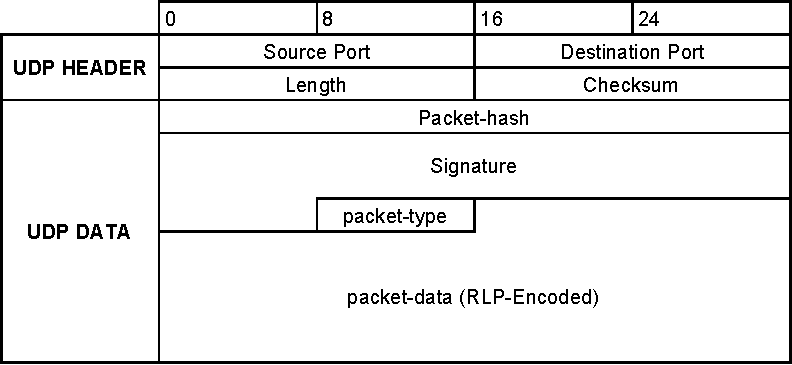
\includegraphics[width=0.7\textwidth]{./res/img/rlp-node-discovery-packet-format.pdf}
    \caption{The structure of an RLPx Node Discovery package.}
    \label{fig:rlpx-node-discovery}
    \end{center}
\end{figure}

The packet format is illustrated in~\autoref{fig:rlpx-node-discovery}.




\subparagraph{Joining the network}
In order to join the network for the first time, a new node should generate a
new public-private key pair\footnote{The public key is the ID and the private
key is used to sign the packets.} and know the contact of at least one
participant. In Ethereum this task is accomplished by hard-coding the contact
information of some \textit{bootstrap nodes} in the client's code. The aim of
these nodes is to provide new nodes with contact information to other regular
nodes that are already participating in the network.

RLPx uses its own URL scheme, the \emph{enode}. In this scheme are specified
the ID
of the node encoded in hexadecimal format, the IP-Address and the TCP-Port of
the node:
\begin{verbatim}
enode://<hexadecimal-node-id>@<IP>:<TCP-Port>[?discport:<UDP-PORT>]
\end{verbatim}
The \verb|discport| part is optional and is required only if the UDP port
(discovery port) does not correspond to the TCP one. The default discovery UDP
port is 30303.

